\section{FMEA}
\begin{figure}[H]
    \centering
    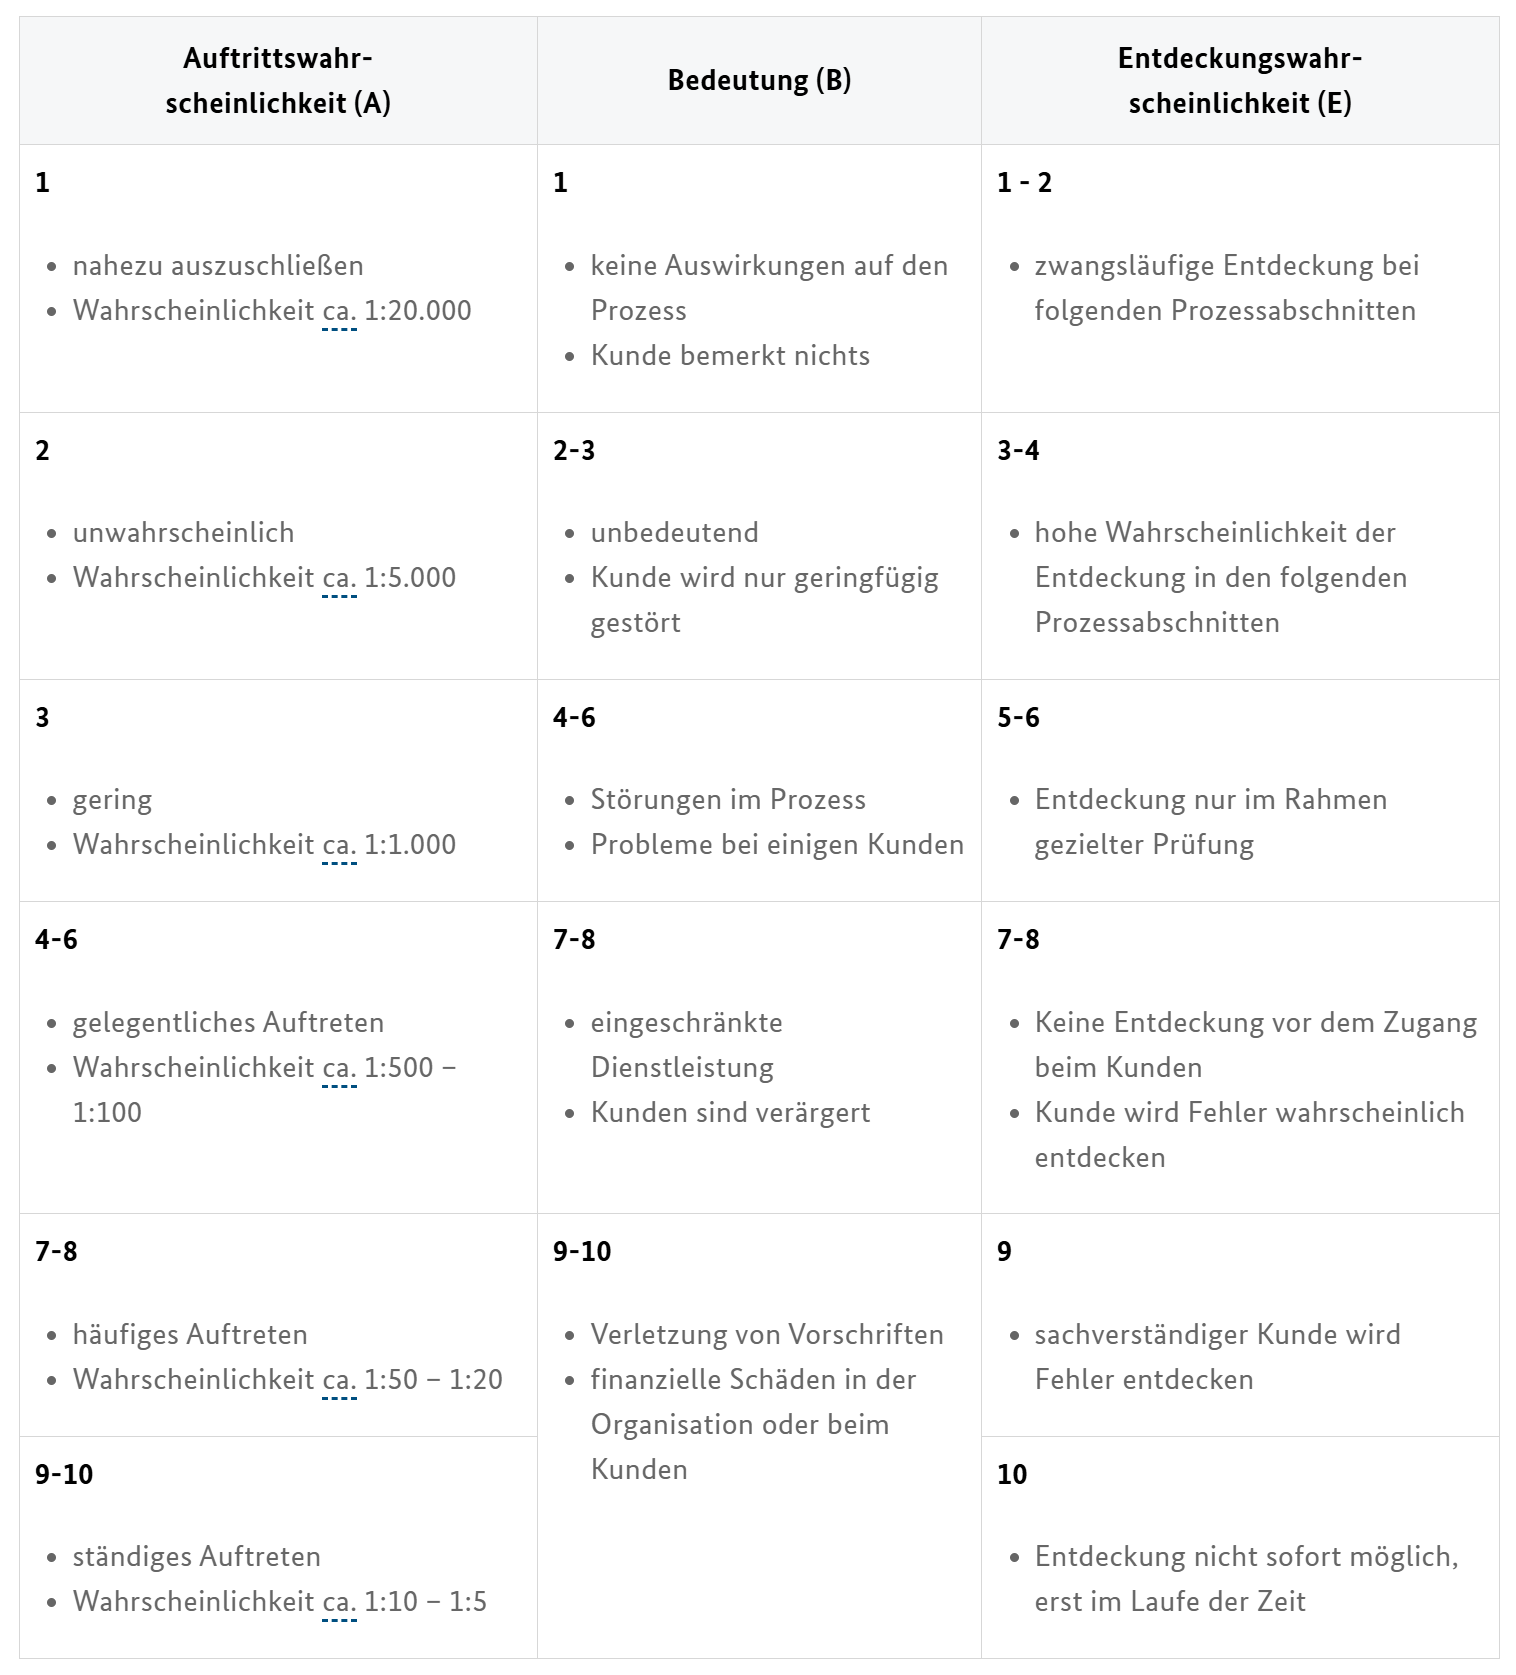
\includegraphics[width=\textwidth]{images/FMEA_2.png}
    \caption{Bewertungsskala der FMEA nach \cite{Bundesministerium_2018}}
    \label{fig:fmea_bewertung}
\end{figure}

\section{Begriffsdefinitionen und relevante Frameworks}
\begin{center}
    \begin{table}[H]
        \begin{tabular}{|p{2.5cm}|p{4.9cm}|p{2.5cm}|p{4.9cm}|}
            \hline
            \textbf{Begriffe} & \textbf{Definitionen} & \textbf{Framework} & \textbf{Erläuterung} \\
            \hline
            Data Governance & Rahmenwerk, um qualitativ hochwertige Daten und die regelkonforme Nutzung sowie Verwahrung sicherstellen zu können \cite{Borus_2020} & ISO & Internationale Organisation für Normungen \\
            \hline
            Overfitting & Überangepasstheit des Modells an Trainingsdaten, sodass mit neuen Datensätzen keine genauen Vorhersagen mehr getroffen werden können \cite{zlobin_data-driven_2025} & ISO 31000 & Internationale Norm zur Identifikation und Vermeidung von Risiken \cite{ISO_2018} \\
            \hline
            Bias & Vorurteile eines Modells aufgrund von homogenen oder veralteten Daten, was zu diskriminierenden Vorhersagen führen kann & ISO 21500 & Liefert Anleitungen für effektives Projektmanagement \cite{ISO_2021} \\
            \hline
            FMEA & Fehlermöglichkeits- und Einflussanalyse \cite{Bundesministerium_2018} & ISO/IEC 27001 - 27008 & Normreihe für Informationssicherheit, beinhaltet Basisnormen ISO 27001-27008 \cite{Kersten_27001_2019} \\
            \hline
            KRI & Key Risk Indicators & PMBOK & Project Management Body of Knowledge, Sammlung von Best Practices für Projektmanagement \cite{noauthor_pmbok_nodate} \\
            \hline
            Safeguards & Maßnahmenlisten, um Risiken vermeiden zu können \cite{Kersten_27001_2019}  & SCRUM & Methode des agilen Projektmanagements, gekennzeichnet durch eine iterative Arbeitsweise \cite{Rubin_2014} \\
            \hline
            Black-Box-Problem & ein Problem, das entsteht, wenn Forschende nicht nachvollziehen können, weshalb neuronale Netzwerke zu ihren Ergebnissen kommen \cite{rai_explainable_2020} & COSO ERM -- Enterprise Risk Management Framework & Sammlung bewährter Methoden für Projekt- und Risikomanagement \cite{COSO_2020} \\
            \hline
            Monte-Carlo-Simulation & Mathematische Technik, um Unsicherheiten in Vorhersagen einbeziehen zu können \cite{gleisner_risikoaggregation_2019} & NIST (AI) Risk Management Framework & US Standard für das Management von KI-Risiken \cite{NIST_2023} \\
            \hline
        \end{tabular}
         \caption{Begriffsdefinitionen und relevante Frameworks, eigene Darstellung}
    \label{fig:begriffsdefinitionen}
    \end{table}
\end{center}

